
%% bare_conf.tex
%% V1.3
%% 2007/01/11
%% by Michael Shell
%% See:
%% http://www.michaelshell.org/
%% for current contact information.
%%
%% This is a skeleton file demonstrating the use of IEEEtran.cls
%% (requires IEEEtran.cls version 1.7 or later) with an IEEE conference paper.
%%
%% Support sites:
%% http://www.michaelshell.org/tex/ieeetran/
%% http://www.ctan.org/tex-archive/macros/latex/contrib/IEEEtran/
%% and
%% http://www.ieee.org/

%%*************************************************************************
%% Legal Notice:
%% This code is offered as-is without any warranty either expressed or
%% implied; without even the implied warranty of MERCHANTABILITY or
%% FITNESS FOR A PARTICULAR PURPOSE! 
%% User assumes all risk.
%% In no event shall IEEE or any contributor to this code be liable for
%% any damages or losses, including, but not limited to, incidental,
%% consequential, or any other damages, resulting from the use or misuse
%% of any information contained here.
%%
%% All comments are the opinions of their respective authors and are not
%% necessarily endorsed by the IEEE.
%%
%% This work is distributed under the LaTeX Project Public License (LPPL)
%% ( http://www.latex-project.org/ ) version 1.3, and may be freely used,
%% distributed and modified. A copy of the LPPL, version 1.3, is included
%% in the base LaTeX documentation of all distributions of LaTeX released
%% 2003/12/01 or later.
%% Retain all contribution notices and credits.
%% ** Modified files should be clearly indicated as such, including  **
%% ** renaming them and changing author support contact information. **
%%
%% File list of work: IEEEtran.cls, IEEEtran_HOWTO.pdf, bare_adv.tex,
%%                    bare_conf.tex, bare_jrnl.tex, bare_jrnl_compsoc.tex
%%*************************************************************************
\documentclass[9pt]{sig-alternate}

%\usepackage{biblatex}
%\usepackage{amsmath}
%\usepackage{amssymb}
%\usepackage{times}
\usepackage{hyperref}
%\usepackage{graphicx}
\usepackage{wrapfig}
\usepackage{listings}
\usepackage[usenames,dvipsnames]{xcolor}
%\usepackage{setspace}
\usepackage{python_syntax}
%\usepackage{bibentry}
\usepackage{todonotes}
\usepackage{url}
\usepackage{lineno}
%\usepackage{natbib}
%\usepackage{caption}
\usepackage[english]{babel} 
\def\UrlFont{\em} % Italicize all URLs.  
\lstset{
	basicstyle=\footnotesize\ttfamily,
	breaklines=true,
	language=Python,
	}
\newcommand{\verbx}[1]{\lstinline{#1}}
\newcommand{\bfhead}[1]{\noindent \textbf{#1:}}

\usepackage{alltt}
\renewcommand{\ttdefault}{txtt}
%%\usepackage{color}
%%\usepackage[usenames,dvipsnames,svgnames,table]{xcolor}
%%\definecolor{mauve}{rgb}{0.58,0,0.82}
%\definecolor{light-gray}{gray}{0.75}
%\usepackage{listings}
%\lstset{
%  language=Python,
%  showstringspaces=false,
%  formfeed=\newpage,
%  tabsize=4,
%  commentstyle=\itshape,
%  basicstyle=\ttfamily\scriptsize,
%  morekeywords={lambda, self, assert, as},
%  numbers=left,
%  numberstyle=\scriptsize\color{light-gray}\textsf,
%  xleftmargin=2em,
%  stringstyle=\color{mauve}
%}
%\lstdefinestyle{Bash}{
%    language={}, 
%    moredelim=**[is][\color{blue}\bf\ttfamily]{`}{`},
%}
%\lstdefinestyle{OpenCL}{
%	language=C++,
%	morekeywords={kernel, __kernel, global, __global, size_t, get_global_id, sin}
%}
%
%\usepackage{float}
%\floatstyle{ruled}
%\newfloat{codelisting}{tp}{lop}
%\floatname{codelisting}{Listing}

% *** GRAPHICS RELATED PACKAGES ***
%
% *** MATH PACKAGES ***
%
%\usepackage[cmex10]{amsmath}
% A popular package from the American Mathematical Society that provides
% many useful and powerful commands for dealing with mathematics. If using
% it, be sure to load this package with the cmex10 option to ensure that
% only type 1 fonts will utilized at all point sizes. Without this option,
% it is possible that some math symbols, particularly those within
% footnotes, will be rendered in bitmap form which will result in a
% document that can not be IEEE Xplore compliant!
%
% Also, note that the amsmath package sets \interdisplaylinepenalty to 10000
% thus preventing page breaks from occurring within multiline equations. Use:
%\interdisplaylinepenalty=2500
% after loading amsmath to restore such page breaks as IEEEtran.cls normally
% does. amsmath.sty is already installed on most LaTeX systems. The latest
% version and documentation can be obtained at:
% http://www.ctan.org/tex-archive/macros/latex/required/amslatex/math/

% *** SPECIALIZED LIST PACKAGES ***
%
%\usepackage{algorithmic}
% algorithmic.sty was written by Peter Williams and Rogerio Brito.
% This package provides an algorithmic environment fo describing algorithms.
% You can use the algorithmic environment in-text or within a figure
% environment to provide for a floating algorithm. Do NOT use the algorithm
% floating environment provided by algorithm.sty (by the same authors) or
% algorithm2e.sty (by Christophe Fiorio) as IEEE does not use dedicated
% algorithm float types and packages that provide these will not provide
% correct IEEE style captions. The latest version and documentation of
% algorithmic.sty can be obtained at:
% http://www.ctan.org/tex-archive/macros/latex/contrib/algorithms/
% There is also a support site at:
% http://algorithms.berlios.de/index.html
% Also of interest may be the (relatively newer and more customizable)
% algorithmicx.sty package by Szasz Janos:
% http://www.ctan.org/tex-archive/macros/latex/contrib/algorithmicx/

% *** ALIGNMENT PACKAGES ***
%
%\usepackage{array}
% Frank Mittelbach's and David Carlisle's array.sty patches and improves
% the standard LaTeX2e array and tabular environments to provide better
% appearance and additional user controls. As the default LaTeX2e table
% generation code is lacking to the point of almost being broken with
% respect to the quality of the end results, all users are strongly
% advised to use an enhanced (at the very least that provided by array.sty)
% set of table tools. array.sty is already installed on most systems. The
% latest version and documentation can be obtained at:
% http://www.ctan.org/tex-archive/macros/latex/required/tools/

%\usepackage{mdwmath}
%\usepackage{mdwtab}
% Also highly recommended is Mark Wooding's extremely powerful MDW tools,
% especially mdwmath.sty and mdwtab.sty which are used to format equations
% and tables, respectively. The MDWtools set is already installed on most
% LaTeX systems. The lastest version and documentation is available at:
% http://www.ctan.org/tex-archive/macros/latex/contrib/mdwtools/

% IEEEtran contains the IEEEeqnarray family of commands that can be used to
% generate multiline equations as well as matrices, tables, etc., of high
% quality.

%\usepackage{eqparbox}
% Also of notable interest is Scott Pakin's eqparbox package for creating
% (automatically sized) equal width boxes - aka "natural width parboxes".
% Available at:
% http://www.ctan.org/tex-archive/macros/latex/contrib/eqparbox/

% *** SUBFIGURE PACKAGES ***
%\usepackage[tight,footnotesize]{subfigure}
% subfigure.sty was written by Steven Douglas Cochran. This package makes it
% easy to put subfigures in your figures. e.g., "Figure 1a and 1b". For IEEE
% work, it is a good idea to load it with the tight package option to reduce
% the amount of white space around the subfigures. subfigure.sty is already
% installed on most LaTeX systems. The latest version and documentation can
% be obtained at:
% http://www.ctan.org/tex-archive/obsolete/macros/latex/contrib/subfigure/
% subfigure.sty has been superceeded by subfig.sty.

%\usepackage[caption=false]{caption}
%\usepackage[font=footnotesize]{subfig}
% subfig.sty, also written by Steven Douglas Cochran, is the modern
% replacement for subfigure.sty. However, subfig.sty requires and
% automatically loads Axel Sommerfeldt's caption.sty which will override
% IEEEtran.cls handling of captions and this will result in nonIEEE style
% figure/table captions. To prevent this problem, be sure and preload
% caption.sty with its "caption=false" package option. This is will preserve
% IEEEtran.cls handing of captions. Version 1.3 (2005/06/28) and later 
% (recommended due to many improvements over 1.2) of subfig.sty supports
% the caption=false option directly:
%\usepackage[caption=false,font=footnotesize]{subfig}
%
% The latest version and documentation can be obtained at:
% http://www.ctan.org/tex-archive/macros/latex/contrib/subfig/
% The latest version and documentation of caption.sty can be obtained at:
% http://www.ctan.org/tex-archive/macros/latex/contrib/caption/

% *** FLOAT PACKAGES ***
%
%\usepackage{fixltx2e}
% fixltx2e, the successor to the earlier fix2col.sty, was written by
% Frank Mittelbach and David Carlisle. This package corrects a few problems
% in the LaTeX2e kernel, the most notable of which is that in current
% LaTeX2e releases, the ordering of single and double column floats is not
% guaranteed to be preserved. Thus, an unpatched LaTeX2e can allow a
% single column figure to be placed prior to an earlier double column
% figure. The latest version and documentation can be found at:
% http://www.ctan.org/tex-archive/macros/latex/base/

%\usepackage{stfloats}
% stfloats.sty was written by Sigitas Tolusis. This package gives LaTeX2e
% the ability to do double column floats at the bottom of the page as well
% as the top. (e.g., "\begin{figure*}[!b]" is not normally possible in
% LaTeX2e). It also provides a command:
%\fnbelowfloat
% to enable the placement of footnotes below bottom floats (the standard
% LaTeX2e kernel puts them above bottom floats). This is an invasive package
% which rewrites many portions of the LaTeX2e float routines. It may not work
% with other packages that modify the LaTeX2e float routines. The latest
% version and documentation can be obtained at:
% http://www.ctan.org/tex-archive/macros/latex/contrib/sttools/
% Documentation is contained in the stfloats.sty comments as well as in the
% presfull.pdf file. Do not use the stfloats baselinefloat ability as IEEE
% does not allow \baselineskip to stretch. Authors submitting work to the
% IEEE should note that IEEE rarely uses double column equations and
% that authors should try to avoid such use. Do not be tempted to use the
% cuted.sty or midfloat.sty packages (also by Sigitas Tolusis) as IEEE does
% not format its papers in such ways.

% *** PDF, URL AND HYPERLINK PACKAGES ***
%
% url.sty was written by Donald Arseneau. It provides better support for
% handling and breaking URLs. url.sty is already installed on most LaTeX
% systems. The latest version can be obtained at:
% http://www.ctan.org/tex-archive/macros/latex/contrib/misc/
% Read the url.sty source comments for usage information. Basically,
% \url{my_url_here}.

%\usepackage{placeins}

% *** Do not adjust lengths that control margins, column widths, etc. ***
% *** Do not use packages that alter fonts (such as pslatex).         ***
% There should be no need to do such things with IEEEtran.cls V1.6 and later.
% (Unless specifically asked to do so by the journal or conference you plan
% to submit to, of course. )


% correct bad hyphenation here
\hyphenation{op-tical net-works semi-conduc-tor}

\begin{document}
%
% paper title
% can use linebreaks \\ within to get better formatting as desired
\title{Collaborative Infrastructure for Test-Driven\\Scientific Model Validation}


% author names and affiliations
% use a multiple column layout for up to two different
% affiliations
\numberofauthors{2}
\author{\alignauthor
Cyrus Omar, Jonathan Aldrich\\\affaddr{Carnegie Mellon University}\\
       \email{\{comar,aldrich\}@cs.cmu.edu}
       \alignauthor Richard C. Gerkin\\
       \affaddr{Arizona State University}\\{rgerkin@asu.edu}
}

% conference papers do not typically use \thanks and this command
% is locked out in conference mode. If really needed, such as for
% the acknowledgment of grants, issue a \IEEEoverridecommandlockouts
% after \documentclass

% for over three affiliations, or if they all won't fit within the width
% of the page, use this alternative format:
% 
%\author{\IEEEauthorblockN{Michael Shell\IEEEauthorrefmark{1},
%Homer Simpson\IEEEauthorrefmark{2},
%James Kirk\IEEEauthorrefmark{3}, 
%Montgomery Scott\IEEEauthorrefmark{3} and
%Eldon Tyrell\IEEEauthorrefmark{4}}
%\IEEEauthorblockA{\IEEEauthorrefmark{1}School of Electrical and Computer Engineering\\
%Georgia Institute of Technology,
%Atlanta, Georgia 30332--0250\\ Email: see http://www.michaelshell.org/contact.html}
%\IEEEauthorblockA{\IEEEauthorrefmark{2}Twentieth Century Fox, Springfield, USA\\
%Email: homer@thesimpsons.com}
%\IEEEauthorblockA{\IEEEauthorrefmark{3}Starfleet Academy, San Francisco, California 96678-2391\\
%Telephone: (800) 555--1212, Fax: (888) 555--1212}
%\IEEEauthorblockA{\IEEEauthorrefmark{4}Tyrell Inc., 123 Replicant Street, Los Angeles, California 90210--4321}}




% use for special paper notices
%\IEEEspecialpapernotice{(Invited Paper)}




% make the title area
\maketitle

\begin{abstract}
One of the pillars of the modern scientific method is \emph{model validation}: comparing a scientific model's predictions against empirical observations. Today, a scientist demonstrates the validity of a model by making an argument in a paper and submitting it for peer review, a process comparable to \emph{code review} in software engineering. While human review helps to ensure that contributions meet high-level goals, software engineers typically supplement it with \emph{unit testing} to get a more complete picture of the status of a project, particularly when it is complex and involves many contributors.

We argue that a similar test-driven methodology would be valuable to scientific communities as they seek to  validate increasingly complex models against growing repositories of empirical data. Scientific communities differ from software communities in several key ways, however. In this paper, we introduce \emph{SciUnit}, a framework for test-driven scientific model validation and outline how SciUnit, supported by new and existing collaborative infrastructure, could be  integrated into the modern scientific workflow.
%in the context of the applications and architectures that the language may need to target.
%
%Programming languages targeted toward end-users in high-performance computing must consider a number of issues in addition to performance. Typically, researchers have focused verifiability, portability and ease-of-use, and the right balance often depends on the particular uses that they are put toward.
%
%Ace %, evaluates it against several design and adoption criteria, and describes several use cases as well as a realistic case study involving parallelizing neurobiological circuit simulations on clusters of GPUs. 
%is an extensible statically-typed programming language embedded within the ubiquitous scripting language Python. Python serves as a {metalanguage}, enabling programmatic control over several aspects of language specification and compilation. 
%We demonstrate the power of this design for HPC by defining all of the primitives of the OpenCL kernel language as a library of user-defined types in Ace, then extending this core with several higher-level first-class abstractions. The target of translation, called the \emph{backend}, is user-defined as well, allowing us to implement the semantics of these primitives by direct translation to OpenCL, CUDA or C99.
%
%Although Ace is built around a static type discipline, it supports a novel form of generic programming based on type propagation that, together with a form of extensible local type inference, eliminates most of the syntactic overhead usually associated with statically-typed languages. A companion host API allows type information from \verb|numpy| arrays to directly propagate into Ace kernels, supporting seamless adoption of Ace into current scientific workflows.
%
\end{abstract}

%\begin{IEEEkeywords}
%unit testing, validation, computer-supported collaborative work
%\end{IEEEkeywords}


% For peer review papers, you can put extra information on the cover
% page as needed:
% \ifCLASSOPTIONpeerreview
% \begin{center} \bfseries EDICS Category: 3-BBND \end{center}
% \fi
%
% For peerreview papers, this IEEEtran command inserts a page break and
% creates the second title. It will be ignored for other modes.
%\IEEEpeerreviewmaketitle

\section{Introduction}
\begin{figure*}[t]
\vspace{-30px}
\centering
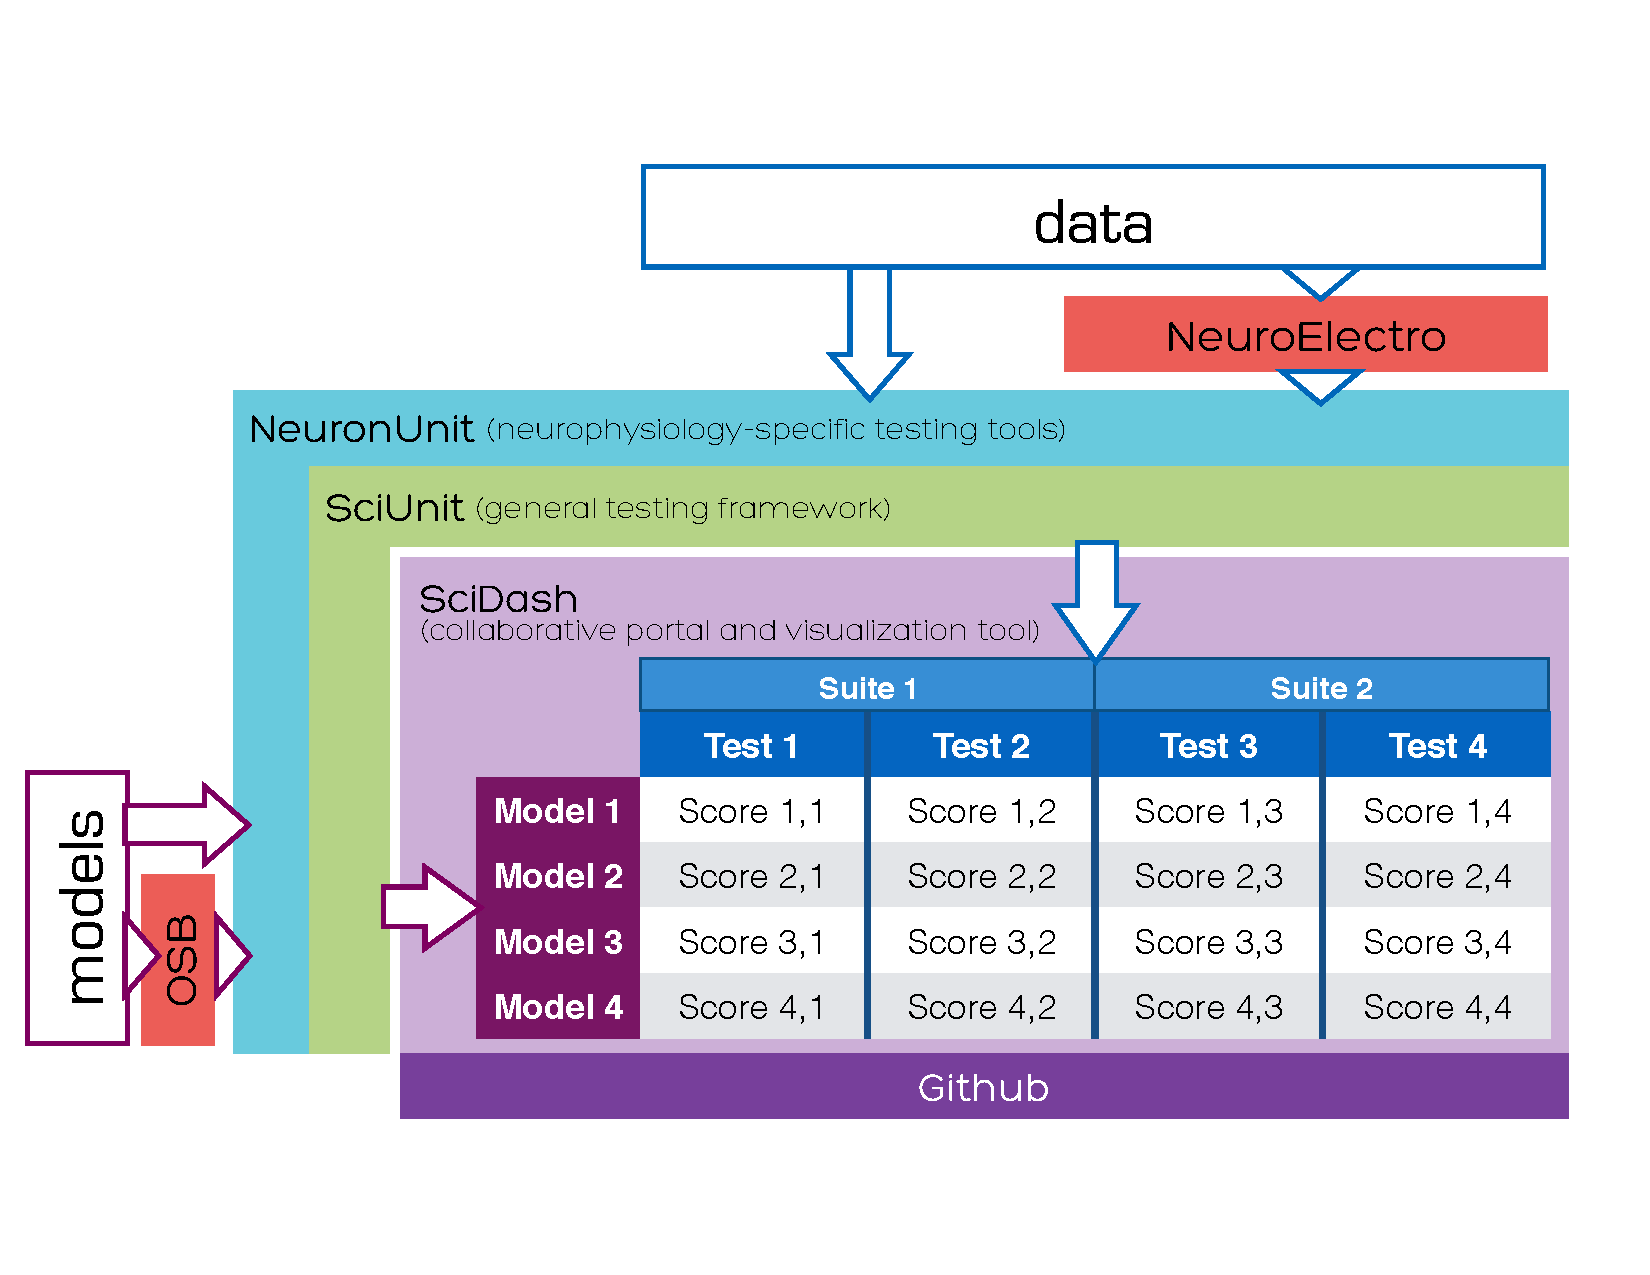
\includegraphics[scale=0.45]{diagram1.pdf}
\vspace{-40px}
\caption{Tests are derived from data and models are derived from scientific theories. The score table summarizes the performance of a collection of models against a suite of tests. A table is contained in a \emph{suite repository} (e.g. \texttt{saturnsuite}), hosted on social coding infrastructure -- here, Github. SciDash is a portal that discovers and organizes these suite repositories  and provides tools for visualizing them. Tests interface with models using capabilities, as specified by the testing framework (\texttt{sciunit}). Common testing code, capabilities and bridges to external model and data repositories are also collaboratively developed (e.g. \texttt{cosmounit}).}  
\label{fig:sciunit_overview}
\end{figure*}


Scientific theories are increasingly being organized around \emph{quantitative models}:  formal systems capable of generating predictions about observable quantities. A model can be  characterized by its \textit{scope}: the set of observable quantities that it attempts to predict, and by its \textit{validity}: the extent to which its predictions agree with experimental observations of these quantities. 

Quantitative models are today validated by \emph{peer review}. For a model to be accepted by a scientific community, its advocates must submit a paper describing how it works and providing evidence that it predicts a quantity of interest more accurately than previous models, or in some cases, that it makes a desirable tradeoff  between accuracy and complexity \cite{box1987empirical}. Other members of the relevant community are then tasked with ensuring that validity was measured properly and that relevant data and competing models were adequately considered, drawing on knowledge of statistical methods and on the prior literature. Publishing is a primary motivator for most scientists \cite{howison2011scientific}.

Quantitative scientific modeling and software development share much in common. Indeed, quantitative models are increasingly being implemented in software and in some cases, the software \emph{is} the model (e.g. complex simulations). The peer review process for papers is similar in many ways to the \emph{code review} process used in many development teams, where team members look for mistakes, enforce style and architectural guidelines and check that the code is \emph{valid} (i.e. that it achieves its intended goal) before permitting it to be committed to the primary source code repository. 


Code review can be quite effective \cite{codereview}, but this requires that developers  expend considerable effort \cite{kemerer2009impact}. 
%Code review is also most effective for resolving  issues related to software architecture. 
Most large development teams thus supplement code reviews with more {automated} approaches to verification and validation, the most widely-used  of which is \emph{unit testing} \cite{beck2003}. In brief, unit tests are functions that check that the output of a single component satisfies a single well-defined  criterion. A suite of such tests can be considered a partial specification of the program or component under development.  Test suites serve as a complement to code review by allowing developers to answer questions like these more easily:
\begin{enumerate}
\item Which functionality has been adequately implemented? What remains to be done?
%\item How much progress does an individual code contribution make? 
\item How does the team measure validity?
\item Does a candidate code contribution cause \emph{regressions} in other parts of a program?
\end{enumerate}
Scientists ask analagous questions:
\begin{enumerate}
\item Which observations are already explained by existing models? What are the best models? What are the open modeling problems of interest?
%\item How much better is a new model than the state of the art? What are the open problems in my field?
\item What are the contemporary community standards for measuring goodness-of-fit?
\item How do newly-made experimental observations impact the validity of previously-published models?
\end{enumerate}
But while software engineers can rely on a program's test suite, scientists today must extract this information from a body of scientific publications. This is increasingly difficult. Each publication focuses on just one model and is frozen in time, so it does not consider the latest experimental data or statistical methods. Discovering, precisely characterizing and comparing models to discover the state of the art and find open modeling problems can require an encyclopedic knowledge of the literature. Senior scientists often attempt to fill this need by publishing review papers, but in many areas, the number of publications generated every year can be overwhelming \cite{jinha_article_2010}, and comprehensive reviews of a particular area are published relatively infrequently. Statisticians often complain that scientists are not following best practices and that community standards evolve too slowly because a canonical paper or popular review used outdated methods. Furthermore, if the literature simply doesn't address an important question of validity, a researcher often needs to reimplement a model from scratch. 

One might compare this to a large software development team relying primarily on carefully prepared and reviewed component documentation together with occasional high-level project summaries produced by the lead architects to answer the questions enumerated above.
Although certainly a caricature, this motivates our suggestion that the scientific process could be improved by the adoption of test-driven methodologies alongside traditional peer review. However, the scientific community presents several unique challenges that must be addressed by any such methodology:
\begin{enumerate}
\item Unit tests are typically pass/fail, while goodness-of-fit between a model and data is typically measured by a continuous metric (e.g. a $p$-value). 
\item Unit tests often test a \emph{particular} component, whereas a \emph{validation test} must be able to uniformly handle any model capable of predicting the quantity being tested. %They are sometimes reluctant to share certain details of their implementations \cite{badscientists}.
%\item Experimental data can itself be erroneous, noisy or inconsistent with other available data.
\item Different modelers often  prefer different programming languages and data structures. Similarly, data formats differ between experimentalists. The validation  testing framework must be flexible about these choices.
\item Professional software developers are typically trained in testing practices and tools, while scientists  rarely have training or experience with testing practices \cite{oai:open.ac.uk.OAI2:17673}. Thus, the framework must be as simple as possible.
\item Different communities, groups and individuals prefer different goodness-of-fit metrics and emphasize different sets of observable quantities. These can evolve as, for example, statisticians develop better measures. In contrast, there is more pressure to agree upon requirements and priorities in a software development project.
\end{enumerate}

To address challenges 1-4, we will introduce a lightweight scientific validation testing framework, \textit{SciUnit}, in Sec. 2. Challenge 5 has to do with coordination between scientists. To address this, we introduce a community workflow based on widely-adopted social coding tools (here Github) along with a lightweight community portal called \textit{SciDash}. The overall goal of this work is to help scientists generate and examine tables like the one central to Figure 1, where the relative validity of a set of models having a common scope can be determined by examining scores produced by a suite of validation tests constructed from experimental data. 

%Anecdotally, one of the greatest fears of new scientists is that a problem that they are working on has already been solved and published. 


%This suggests that tools that help researchers answer questions like these could help readers and reviewers develop a more comprehensive understanding of the state-of-the-art and improve the quality of the research being published as a result: to renewed calls for tools that help researchers . 

%These questions are particularly relevant for young scientists and  scientists aiming to enter a new research area to answer.

%understanding of the state-of-the-art from publications containing only a few pieces of data, and then only that data available at the time of publication. 

%These demonstrations also quickly go out of date. Finally, there is no easy way to summarize and compare the claims being made in modeling papers in order to synthesize an understanding of a research area as a whole. 
%A strength of publications are their focused descriptions of new data and models. 
%A weakness, however, is that evaluating the scope and validity of models against known data is intractable using a body of publications alone.

%publications would be analagous to user manuals, rather than rigorous justifications that a program meets a specific specification. Unit tests serve this purpose for software, so we argue that the validation of neuroscience models by means of executable tests would be useful to scientists as a supplement the publication system.
% In addition to this open testing toolkit we also provide a library of tests for models of spiking single neurons.  

% Section 2.
\section{Validation Testing with {SciUnit}}
\begin{figure}[t]
\small
\begin{python}
class PositionTest(sciunit.Test):
    """Tests a planetary position model based on positions observed on day n given the positions in the n-1 previous days.
    Metric: Standard p-value.
    Parameters: 
      obs_histories : list[list[position]]
      obs_positions: list[position]"""
	def __init__(self, obs_histories, obs_positions):
		self.obs_histories = obs_histories
		self.obs_positions = obs_positions

	required_capabilities = [PredictsPlanetaryPosition]

	def _judge(self, model):
		predictions = []
		for obs_history in self.obs_histories:
			predictions.append(model.predict_next_pos(obs_history))
		p = pooled_p_val(predictions, self.obs_positions)
		return sciunit.PValue(p, related_data={
			'obs_histories': obs_histories,
			'obs_positions': obs_positions,
			'predictions': predictions
		})
\end{python}
\vspace{-5px}
\caption{An example test class in \texttt{cosmounit}.}
\label{fig:rate_test}
\vspace{-15px}
\end{figure}

%Simple executable \emph{validation tests} that compute agreement between a model prediction and an experimental observation.  
As a motivating example, we will begin by considering a community of early cosmologists recording and attempting to model observations of the planets visible in the sky, such as their position, velocity, orbital eccentricity and so on. One simple validation test might ask a model to predict planetary position on night $n+1$ given observations of its position on $n$ previous nights. Figure 2 shows how to implement a test, using  SciUnit, that captures this logic.

Before explaining the details of this example, we point out that SciUnit is implemented in Python. Python is one of the most widely used languages in science today \cite{sanner1999python}, and has become the de facto language of open source scientific computing. It supports calling into  many of the other popular languages, including R, MATLAB, C and Java, more cleanly than these languages support calling into Python (challenge 3). It is widely-recognized as being easy-to-read and its object system can be used to define abstract interfaces, which we leverage in support of challenge 2. Alternative implementations of SciUnit, including language-independent specifications of its structure, may be part of future work.  

A \textit{SciUnit} validation test is an {instance} of a Python class implementing the \verbx{sciunit.Test} abstract interface (line 1). 
Here, the class \verbx{PositionTest} takes two \emph{parameters} in its constructor (constructors are named \verbx{\_\_init\_\_} in Python, lines 7-9). 
The meaning of each parameter along with a description of the goodness-of-fit metric used by the test is documented on lines 2-6. 
%For convenience, we also make use of functions provided by the popular NumPy\cite{numpy_url} and SciPy\cite{scipy_url} libraries, although these are not required by \textit{SciUnit}.  
To create a \emph{particular} position test, we instantiate this class with particular planetary observations. 
For example, the subset of cosmologists interested specifically in Saturn might instantiate a test by randomly chunking observations made about Saturn as follows:
\begin{python}
  h, p = randomly_chunk(saturn_obs_positions)
  saturn_position_test = SpikeCountTest(h, p)
\end{python}

The class \verb|PositionTest| defines logic that is not specific to any particular planet, so it is contained in a package shared by all cosmologists called \verbx{cosmounit}, while the particular test above would be used in a test suite focused specifically on Saturn called \verbx{saturnsuite}. Both the common logic and specific suites are collaboratively developed by these overlapping research communities in source code repositories on Github (or another similar service).

Classes that implement the \verbx{sciunit.Test} interface must contain a \verbx{_judge} method that receives a candidate \emph{model} as input and produces a \textit{score} as output. 
To specify the interface between the test and the model, the test author provides a list of \emph{capabilities} in the \verbx{required_capabilities} attribute, seen on line 11 of Fig. \ref{fig:rate_test}. 
Capabilities are simply collections of methods that a test will need to invoke in order to receive relevant data, and are analogous to \emph{interfaces} in e.g. Java. 
In Python, capabilities must be written as classes with unimplemented members. 
The capability required by the test in Figure \ref{fig:rate_test} is shown in Figure \ref{fig:capability}. 
In \textit{SciUnit}, classes defining capabilities are tagged as such by inheriting from \verbx{sciunit.Capability}. The test in Figure \ref{fig:rate_test} repeatedly uses this capability on line 16 to produce a position prediction for each observation.  We assume that positions are represented in a standardized manner specified within \verbx{cosmounit}. A model is simply an object that implements capabilities (via Python's simple inheritance mechanism).

The remainder of the \verbx{_judge} method compares the model predictions to observed data to produce a pooled $p$ value. The method returns an instance of \verbx{sciunit.PValue}, a subclass of \texttt{sciunit.Score} that has been included with \textit{SciUnit} due to its generality. In addition to the $p$-value itself, the returned score object also contains metadata, via the \verbx{related_data} parameter, for  scientists who may wish to examine the result in more detail later. This illustrates some key differences between unit testing, which would simply produce a boolean result, and our conception of scientific validation testing (challenge 1). A score must induce an ordering, so that the table shown in Figure 1 can be sorted along its columns, and it can optionally specify a normalization scheme so the cells can be color-coded (not shown). A test can be manually executed using the \verbx{judge} method:
\begin{python}
score = saturn_position_test.judge(kepler_sat)
\end{python}

This method proceeds by first checking that the provided model implements all required capabilities before calling the test's \verbx{_judge} method to produce a score. A reference to the test and model are added to the score for convenience (accessible via the \verbx{test} and \verbx{model} attributes, respectively).

Alongside this position test, we could also provide a number of other test classes in \verbx{cosmounit} and instantiate them with data about aspects of Saturn's motion (e.g. it's velocity)  to produce a comprehensive suite in \verbx{saturnsuite}. 
\begin{python}
saturn_motion = sciunit.TestSuite([saturn_position_test, saturn_velocity_test, ...])
\end{python}
Like a single test, a test suite is capable of judging one or more models. The result is a score matrix much like the one diagramed in Fig. \ref{fig:sciunit_overview}.
\begin{python}
sm_matrix = saturn_motion.judge([copernicus_sat, ptolemy_sat, newton_sat, kepler_sat])
\end{python}
A test suite requires the union of the capabilities required by the tests it contains. A model that performs well across tests in such a suite could reasonably claim (e.g. to reviewers) that it is a coherent, valid model of Saturn's motion. As new data is collected, new tests can be added to the suite. However, because the interface between the test and the model remains the same (only the data parameterizing the tests changes), the table can be updated automatically. Similarly, when a new model is developed, it can immediately be evaluated against all known data that has been encoded as a test by simply exposing its predictions via the capabilities the test requires. %They then defined a combined metric favoring models that broadly succeeded at meeting these criteria, to produce an overall ranking. 
%Such combined criteria are simply validation tests that invoke other tests to produce a result.
 
%In many cases, models require no modifications to take the new tests because the same type of model output is being requested.
%We discuss visualization of results in Secs. \ref{sec:scidash_activities} and \ref{sec:scidash_visualization}.

\begin{figure}
\begin{python}
class PredictsPlanetaryPosition(sciunit.Capability):
  def predict_next_pos(self, history): 
    """Takes a list of previous positions and produces the next position."""
    raise NotImplementedError("Model does not implement capability.")
\end{python}
\caption{An example capability specifying a single required method (used by the test in Figure \ref{fig:rate_test}).}
\label{fig:capability}
\vspace{-10px}
\end{figure}

%\begin{figure}
%\begin{python}
%class TrainSpikeCountFromCurrent(sciunit.Capability):
%  def train_with_currents(self, currents, counts):
%    """Takes a list of numpy arrays containing current stimulus (in nA) and
%    observed spike counts. Model parameters should be adjusted based on this
%    training data."""
%    raise NotImplementedError("Model does not implement capability.")
%\end{python}
%\caption{Another capability specifying a training protocol (not used by the test in Figure \ref{fig:rate_test}).}
%\label{fig:training}
%\vspace{-15px}
%\end{figure}

%\subsection{Models}
%Capabilities are \emph{implemented} by models. In \textit{SciUnit}, models are instances of Python classes that inherit from \verbx{sciunit.Model}. Like tests, the class itself represents a family of models, parameterized by the arguments of the constructor. A particular model is an instance of such a class.
%
%Figure \ref{fig:simple_model} shows how to write a simple {family} of models, \verbx{LinearModel}, that implement the capability in Fig. \ref{fig:capability} as well as another capability shown in Fig. \ref{fig:training}, which we will discuss below. 
%Models in this family generate a spike count by applying a linear transformation to the mean of the provided input current. The family is parameterized by the scale factor and the offset of the transformation, both scalars. 
%To create a \emph{particular} linear model, a modeler can provide particular parameter values, just as with test families:
%\begin{python}
%CA1_linear_model_heuristic = LinearModel(3.0, 1.0)
%\end{python}
%Here, the parameters to the model were picked by the modeler heuristically, or based on externally-available knowledge. 
%An alternative test design would add a training phase where these parameters were fit to data using the capability shown in Fig. \ref{fig:training}. 
%This test could thus only be used for those models for which parameters can be adjusted without human involvement. 
%Whether to build a training phase into the test protocol is a choice left to each test development community. 
%
%Fig. \ref{fig:rate_test} does not include a training phase. 
%If training data is externally available, models that nevertheless do implement a training capability (like \verb|LinearModel|) can simply be trained explicitly by calling the capability method just like any other Python method:
%\begin{python}
%CA1_linear_model_fit = LinearModel()
%CA1_linear_model_fit.train_with_currents(CA1_training_in, CA1_training_out)
%\end{python}
%\begin{figure}
%\begin{python}
%class LinearModel(sciunit.Model, SpikeCountFromCurrent, 
%    TrainSpikeCountFromCurrent):
%  def __init__(self, scale=None, offset=None): 
%    self.scale, self.offset = scale, offset
%    
%  def spike_count_from_current(self, input):
%    return int(self.scale*numpy.mean(input) + self.offset)
%
%  def train_with_currents(self, currents, counts):
%    means = [numpy.mean(c) for c in currents]
%    [self.offset, self.scale] = numpy.polyfit(means, counts, deg=1)    
%\end{python}
%\caption{A model that returns a spike count by applying a linear transformation to the mean input current. The parameters can be provided manually or learned from data provided by a test or user (see text).}
%\label{fig:simple_model}
%\vspace{-15px}
%\end{figure}
%
\section{Collaborative Workflow}
The design just described has been purposefully left as simple as possible, in pursuit of challenge 4. Despite its simple design, it captures the essential elements of the scientific model validation process and satisfies the four challenges we laid out. SciUnit can be used by individual scientists to organize their workflows, but because science, and in particular, model validation is a collaborative process, we have also described the intended use of SciUnit within a collaborative workflow, mediated by a social coding tool like Github. 

More directly: we anticipate common testing logic (e.g. \verbx{PositionTest}), modeling logic and capabilities being collaboratively developed by larger communities in less specialized repositories like \verbx{cosmounit}. Individuals and small groups will then parameterize these tests and models with data they have gathered, as well as data known from the literature and data contained in existing data repositories to create test suites in repositories like \verbx{saturnsuite}. The interface between data collection software and existing data representation standards and tests will be mediated by bridge logic also contained in repositories like \verbx{cosmounit}.  % This workflow is meant to evoke the \emph{test-driven development} methodology that is often used in software projects. 

Statisticians wishing to promote new validation metrics can simply for a $X$\verbx{unit} repository and implement new test logic. By reusing the same interfaces as previous tests used, these new metrics can immediately be used to validate or invalidate a large body of existing models, providing valuable data for use in convincing the community to adopt these into the mainstream repositories. Similarly, investigators who wish to de-emphasize or emphasize different quantities can fork $X$\verbx{suite} repository and add or remove tests.

To help organize these repositories, a simple collaborative portal sitting above Github called \textit{SciDash} is currently under development (\url{http://scidash.org/}). SciDash consists of an organized, collaboratively filtered listing of $X$\verbx{unit} and $X$\verbx{suite} repositories. That is, it is a tool to help scientists find the most popular repositories in their research area, to facilitate the development of community standards. SciDash also supports extracting summaries of tests, models, scores and related data from suite repositories to generate hyperlinked score tables and documentation. This facilitates exploratory workflows. To modify a suite (e.g. by adding the model a scientist is developing to it), a scientist can simply fork the repository. SciDash automatically discovers public forks of repositories that it is already indexing.
 
\section{Discussion}
Academic peer review and code review are similar, but software developers typically supplement human review with test-driven methodologies. Such methodologies may benefit scientific communities as well, but several unique  constraints make reusing existing testing frameworks and processes difficult. We describe a core testing framework that addresses these issues  by using an existing, widely-adopted language and designing a flexible, simple framework that captures the domain-specific structure of scientific model validation. We then describe, by example, how the various components can be organized into software repositories and collaboratively maintained using social coding tools to support existing scientific practices. We end by outlining a collaboratively filtered portal that sits atop these tools and facilitates exploratory analyses and repository discovery. 

While we discuss a toy example based on planetary movement here, we have applied this framework to more realistic problems in neurobiology in a project called NeuronUnit (http://github.com/scidash/neuronunit). We have used this as part of a collaboration with a large-scale neuroinformatics project (http://www.opensourcebrain.org), whose developers are enthusiastic about a practical pipeline for testing the dozens of models they currently maintain. Much future work remains to be done to investigate whether these tools are truly usable and useful to scientific communities, to further develop the community workflow and infrastructure and to develop a range of realistic case studies. Nevertheless, we believe that identifying the synergies between testing practices and model validation, and describing the basic tooling, represents a novel contribution to the literature on software testing. The core SciUnit framework has been fully developed and is available at http://sciunit.scidash.org/. SciDash is under active development, and is currently capable of basic forms of the operations described in Sec. 3. 

We also plan to use SciUnit to implement competitions among classes of models or techniques in particular subfields. Typically such competitions use \emph{ad hoc} infrastructure. A common framework could be used to make designing and continuously operating such contests more feasible. 

%Modeling competitions in neuroscience, for example, are typically organized around a collection of simple validation criteria, implemented as executable tests. 
%These competitions continue to drive important advances and improve scientists' understanding of the relative merits of different models. 
% \begin{figure}%{r}{0.6\textwidth}
% %\vspace{-38px}
% \includegraphics[scale=0.75]{sciunit_overview.pdf}
% \caption{Proposal overview. 
% \small{i) The \textit{SciUnit} framework can generate discipline-specific libraries for tests generation and model interfacing.  
% \textit{NeuronUnit} is proposed and described here.  Experimental data guides test development; model generation informs and is informed by these \textit{SciUnit} libraries.  
% Each \text{SciUnit} test suite repository on GitHub is indexed by the \textit{SciDash} web application.  
% Test suites for OSB and QSNMC (described in the text) are being built. 
% \textit{SciDash} automatically runs the test collections in each suite and publicly displays the results.}}
% %\vspace{-10px}
% \label{fig:sciunit_overview}
% \end{figure}
% \leavevmode
% \vspace{-0px}

%Each of these examples has leveraged \emph{ad hoc} infrastructure to support test generation. 
%While the specific criteria used to evaluate models varies widely between disciplines in neuroscience, the underlying test-driven methodology has many common features that could be implemented once. 
%Recognizing this, we developed a discipline-agnostic framework for developing scientific validation test suites called \textit{SciUnit} (\url{http://www.sciunit.org}). 

\section*{Acknowledgements}
We thank Sharon Crook, Shreejoy Tripathy and Padraig Gleeson for their support of this project.  
The work was supported in part by grant R01MH081905 from the National Institute of Mental Health. 
The content is solely the responsibility of the authors and does not necessarily represent the official views of the National Institutes of Health.

% conference papers do not normally have an appendix


% use section* for acknowledgement
% trigger a \newpage just before the given reference
% number - used to balance the columns on the last page
% adjust value as needed - may need to be readjusted if
% the document is modified later
%\IEEEtriggeratref{8}
% The "triggered" command can be changed if desired:
%\IEEEtriggercmd{\enlargethispage{-5in}}

% references section

% can use a bibliography generated by BibTeX as a .bbl file
% BibTeX documentation can be easily obtained at:
% http://www.ctan.org/tex-archive/biblio/bibtex/contrib/doc/
% The IEEEtran BibTeX style support page is at:
% http://www.michaelshell.org/tex/ieeetran/bibtex/
%\bibliographystyle{IEEEtran}
% argument is your BibTeX string definitions and bibliography database(s)
%\bibliography{IEEEabrv,../bib/paper}
%
% <OR> manually copy in the resultant .bbl file
% set second argument of \begin to the number of references
% (used to reserve space for the reference number labels box)
\bibliographystyle{IEEEtran}
\bibliography{../research,references,references_crook,urls,references_ja}
%\bibliography{references,references_crook,urls,references_ja}

%\bibliographystyle{unsrt}
%\bibliography{references,references_crook,urls,references_ja}
%\listoftodos
%\end{document}


%
%\begin{thebibliography}{1}
%
%\bibitem{IEEEhowto:kopka}
%H.~Kopka and P.~W. Daly, \emph{A Guide to \LaTeX}, 3rd~ed.\hskip 1em plus
%  0.5em minus 0.4em\relax Harlow, England: Addison-Wesley, 1999.
%
%\end{thebibliography}




% that's all folks
\end{document}


